\chapter{Anhang}\label{chap:appendix}
Das gesamte Projekt liegt öffentlich auf meinem privaten GitHub-Account. \cite{deepvisionProjectGitHub}

Um PreTrained Gewichte und die Gewichte des Trainings herunterzuladen mus \textit{git lfs} installiert sein.
Die Schritte schauen folgendermaßen aus:
\begin{itemize}
	\item git clone <repo>
	\item cd repo\_name
	\item git lfs pull
\end{itemize}

\section{Ordnerstruktur}
\begin{figure}[h]
	\centering
	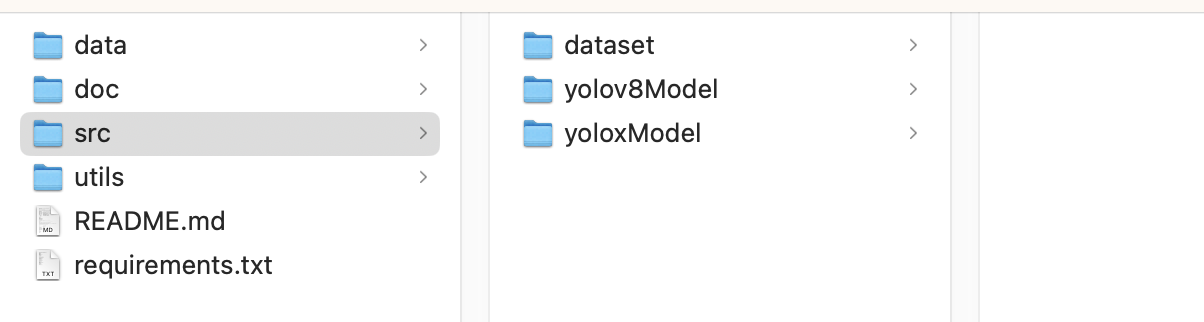
\includegraphics[width=0.55\linewidth]{folder_src.png}
	\caption[Ordnerstruktur des GitHub Repositories]{Ordnerstruktur des GitHub Repositories. Quelle: Eigne Aufnahme}
\end{figure}

\begin{itemize}
	\item data: Darin liegen die Datensätze (in GitHub nicht mit hochgeladen).
	\begin{itemize}
		\item dataFiltered: Der gefilterte Datensatz (nicht annotierte Bilder gelöscht, Klassen zusammengefügt, Train/Val/Test split) mit \textit{datasetPreprocessing.ipynb}
		\item dataRaw: Der unbearbeitete Datensatz \cite{datasetSelfDrivingCar}
		\item dataYolov8: Der Datensatz im Format für YOLOv8 mit \textit{datasetConvertion.ipynb}
		\item dataYoloX:  Der Datensatz im Format für YOLOX mit \textit{datasetConvertion.ipynb}
	\end{itemize}
	\item doc: Dort liegt die Dokumentation im LaTex-Format
	\item src: Dort liegen die Skripte (Datenvorverarbeitung, YOLOX, YOLOv8)
	\item utils: GitHub Repository von YOLOX
	\item requirements.txt: Datei für die Installation der Pakete mit \textit{pip}
\end{itemize}

\section{Dateien: Datensatz}
\begin{figure}[h]
	\centering
	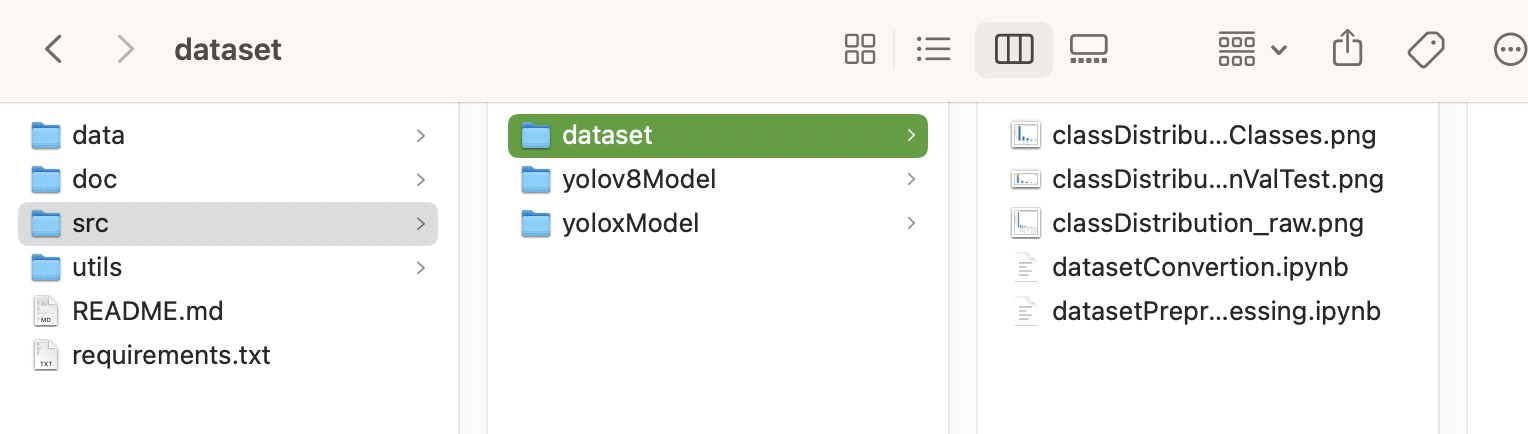
\includegraphics[width=0.55\linewidth]{folder_dataset.png}
	\caption[Ordnerstruktur des src/dataset Ordners.]{Ordnerstruktur des src/dataset Ordners. Quelle: Eigne Aufnahme}
\end{figure}

\begin{itemize}
	\item datasetConvertion.ipynb: Skript zur Umwandlung der Daten in die Formate der Netzwerke
	\item datasetPreprocessing.ipynb: Skript zur Vorverarbeitung des Datensatzes
\end{itemize}



\section{Dateien: YOLOX}
\begin{figure}[h]
	\centering
	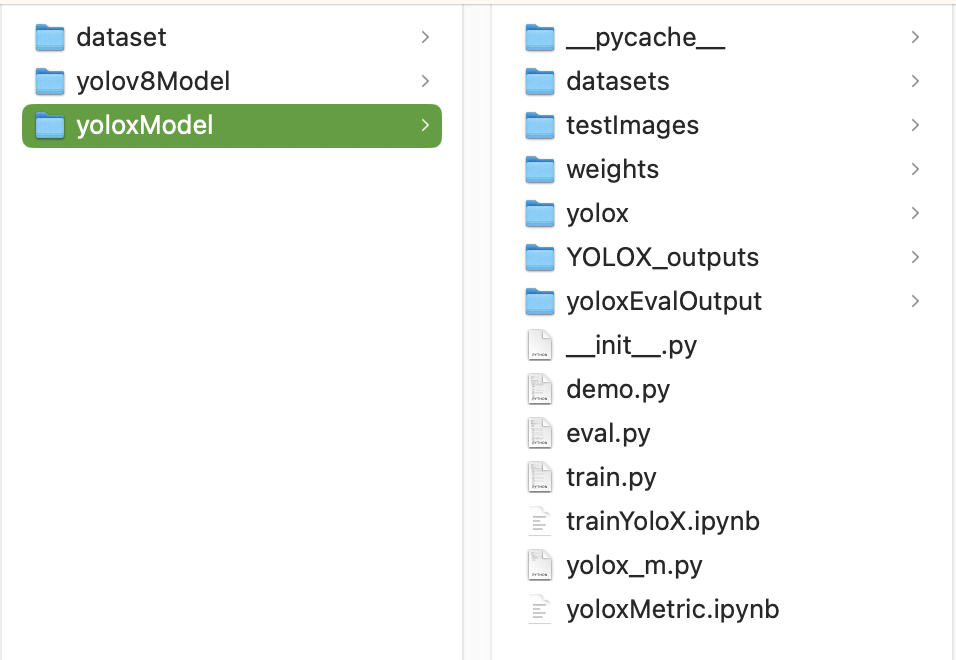
\includegraphics[width=0.55\linewidth]{folder_yolox.png}
	\caption[Ordnerstruktur des src/dataset Ordners.]{Ordnerstruktur des src/dataset Ordners. Quelle: Eigne Aufnahme}
\end{figure}

\begin{itemize}
	\item datasets: Dort liegt der Datensatz im YOLOX Format (Kopie von ./dataset/dataYoloX)
	\item testImages: Vier Testdateien aus dem Testdatensatz
	\item weights: Initialisierungsgewichte aus COCO-Training
	\item yolox: Das yolox-Netzwerk aus den GitHub Repository \cite{yoloxGitHubRepo}
	\item YOLOX\_ouputs: Ausgabe nach dem Training (Gewichte, Log, Visualisierung, ...)
	\item yoloxEvalOutput: Ausgabe im json-Format für die Evaluierung
	\item demo.py: Um das Netzwerk auszuführen auf Eingabebild (aus dem GitHub Repository \cite{yoloxGitHubRepo})
	\item eval.py: Um das Netzwerk zu evaluieren (aus dem GitHub Repository \cite{yoloxGitHubRepo})
	\item train.py: Um das Netzwerk zu trainieren (aus dem GitHub Repository \cite{yoloxGitHubRepo})
	\item trainYoloX.ipynb; Sammlung der Befehle um Netzwerk zu trainieren/evaluieren/auszuführen
	\item yolox\_m.py: Konfiguration des Netzwerks
	\item yoloxMetric.ipynb: Metriken zur Evaluierung berechnen
\end{itemize}

\section{Dateien: YOLOv8}
\begin{figure}[h]
	\centering
	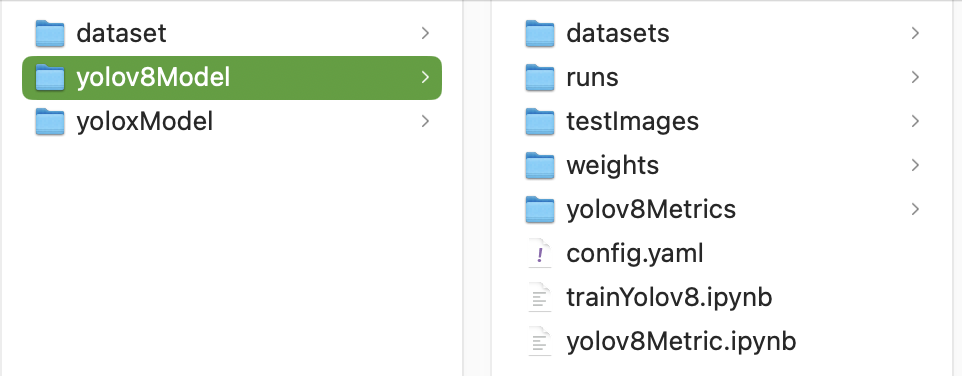
\includegraphics[width=0.55\linewidth]{folder_yolov8.png}
	\caption[Ordnerstruktur des src/dataset Ordners.]{Ordnerstruktur des src/dataset Ordners. Quelle: Eigne Aufnahme}
\end{figure}

\begin{itemize}
	\item datasets: Dort liegt der Datensatz im YOLOv8 Format (Kopie von ./dataset/dataYolov8)
	\item runs: Ausgabe nach dem Training (Gewichte, ...)
	\item testImages: Vier Testdateien aus dem Testdatensatz
	\item weights: Initialisierungsgewichte aus COCO-Training
	\item yolov8Metrics: Dateien zur Evaluierung des Netzwerks
	\item config.yaml:  Konfiguration des Netzwerks
	\item trainYolov8.ipynb: Training des Netzwerks
	\item yolov8Metric.ipynb: Metriken zur Evaluierung berechnen
\end{itemize}